\documentclass[11pt]{article}

\usepackage[letterpaper,margin=0.85in]{geometry}
\usepackage[T1]{fontenc}
\usepackage[utf8]{inputenc}
\usepackage{lmodern}
\usepackage{microtype}
\usepackage{graphicx}
\usepackage{booktabs}
\usepackage{tabularx}
\usepackage{longtable}
\usepackage{array}
\usepackage{enumitem}
\usepackage{xcolor}
\usepackage{hyperref}
\usepackage{fancyhdr}
\usepackage{titlesec}
\usepackage{tcolorbox}
\usepackage{tikz}
\usetikzlibrary{positioning}
\usepackage{siunitx}
\usepackage{amsmath}
\usepackage{amssymb}
\usepackage{csquotes}
\usepackage[backend=biber,style=ieee,sorting=none,maxbibnames=6]{biblatex}
\addbibresource{references.bib}

\definecolor{navy}{HTML}{17365D}
\definecolor{slate}{HTML}{4F5B66}
\definecolor{lightblue}{HTML}{EDF4FA}
\definecolor{lightgray}{HTML}{F4F5F7}
\definecolor{green}{HTML}{2E6B57}
\definecolor{amber}{HTML}{8B6418}

\hypersetup{
  colorlinks=true,
  linkcolor=navy,
  citecolor=navy,
  urlcolor=navy,
  pdfauthor={Jeonghyun Jane Park},
  pdftitle={Sustainable Material Selection for Fused Filament Fabrication in Assistive-Device Prototyping}
}

\pagestyle{fancy}
\fancyhf{}
\lhead{\small Sustainable FFF Materials for Assistive Devices}
\rhead{\small Jeonghyun ``Jane'' Park}
\cfoot{\thepage}
\renewcommand{\headrulewidth}{0.4pt}

\titleformat{\section}{\Large\bfseries\color{navy}}{\thesection}{0.6em}{}
\titleformat{\subsection}{\large\bfseries\color{slate}}{\thesubsection}{0.6em}{}
\titlespacing*{\section}{0pt}{1.4em}{0.6em}
\titlespacing*{\subsection}{0pt}{1.0em}{0.35em}

\setlist[itemize]{leftmargin=1.35em,itemsep=0.2em,topsep=0.3em}
\setlist[enumerate]{leftmargin=1.5em,itemsep=0.25em,topsep=0.3em}
\setlength{\parindent}{0pt}
\setlength{\parskip}{0.55em}
\renewcommand{\arraystretch}{1.22}

\newcolumntype{Y}{>{\raggedright\arraybackslash}X}
\newcolumntype{C}[1]{>{\centering\arraybackslash}p{#1}}

\newtcolorbox{keybox}[1]{
  colback=lightblue,
  colframe=navy,
  boxrule=0.6pt,
  arc=2pt,
  title=\textbf{#1},
  coltitle=navy,
  fonttitle=\bfseries,
  before skip=0.8em,
  after skip=0.8em
}

\newtcolorbox{cautionbox}[1]{
  colback=lightgray,
  colframe=slate,
  boxrule=0.5pt,
  arc=2pt,
  title=\textbf{#1},
  coltitle=slate,
  fonttitle=\bfseries,
  before skip=0.8em,
  after skip=0.8em
}

\begin{document}

% ---------------- COVER ----------------
\begin{titlepage}
\thispagestyle{empty}
\vspace*{0.9in}

{\color{navy}\rule{\textwidth}{1.2pt}}\\[0.45in]

{\Huge\bfseries\color{navy}
Sustainable Material Selection for\\[0.12in]
Fused Filament Fabrication in Custom Assistive Technology\\[0.12in]
}\vspace{0.18in}

{\LARGE\bfseries
A Critical Engineering Review and Decision Framework\\[0.12in]
}

\vspace{0.25in}
{\large\color{slate}
PLA, recycled PET-based feedstocks, PHA, process sustainability, and food-waste-derived composite concepts
}

\vspace{0.6in}

\begin{tcolorbox}[colback=lightblue,colframe=navy,boxrule=0.7pt,arc=2pt,width=0.92\textwidth]
\textbf{Portfolio revision of an internship technical review.} The original report evaluated eco-friendly FFF materials, life-cycle impacts, print emissions, end-of-life pathways, and a food-waste-derived filament concept. This revision expands the original internship review into a graduate-level critical engineering synthesis. It adds an explicit evidence-appraisal method, manufacturing--structure--property analysis, service-normalized life-cycle reasoning, a constraint-based multi-criteria decision framework, uncertainty and sensitivity analysis, and a verification plan grounded in current standards and literature.
\end{tcolorbox}

\vfill

\begin{tabular}{@{}ll@{}}
\textbf{Author:} & Jeonghyun ``Jane'' Park \\
\textbf{Program:} & B.S.E. Mechanical and Aerospace Engineering, Princeton University \\
\textbf{Project context:} & Humanos 3D -- 3D Printing \& Assistive Technology Internship \\
\textbf{Location:} & Medell\'{i}n, Colombia \\
\textbf{Original report:} & August 15, 2025 \\
\textbf{Portfolio revision:} & October 2026 \\
\end{tabular}

\vspace{0.4in}
{\color{navy}\rule{\textwidth}{1.2pt}}
\end{titlepage}

\begin{abstract}
Material-extrusion additive manufacturing offers unusual value for custom assistive technology because it can convert a user-specific functional requirement into a low-volume physical device without dedicated tooling. Sustainability claims for this workflow, however, are often reduced to feedstock labels such as ``bio-based,'' ``recycled,'' or ``compostable.'' This review develops a more rigorous engineering framework for material selection by integrating life-cycle assessment (LCA), FFF process mechanics, user-centered assistive-technology evidence, indoor-emission controls, circularity, and service-life considerations. Three material families are emphasized: polylactic acid (PLA), PETG and recycled PET-based feedstocks, and polyhydroxyalkanoates (PHA). The review also reframes a food-waste-derived composite filament concept as a research hypothesis requiring rheological, mechanical, emissions, energy, and LCA validation rather than as a demonstrated sustainability solution. A key contribution is a decision structure that separates hard feasibility constraints from weighted preferences and evaluates material choices under uncertainty in service life, printing yield, electricity intensity, and end-of-life access. The resulting conclusion is deliberately conditional: no filament is globally sustainable independent of geometry, processing, use conditions, and local infrastructure. For assistive devices, the most defensible material is the one that satisfies functional and safety constraints while minimizing service-normalized burden over a realistic device lifetime.

\textbf{Keywords:} fused filament fabrication; additive manufacturing; assistive technology; PLA; PETG; recycled polymer; PHA; life-cycle assessment; circularity; user-centered design
\end{abstract}

\newpage
\pagenumbering{roman}
\tableofcontents
\newpage

% ---------------- EXEC SUMMARY ----------------
\section*{Executive Summary}
\addcontentsline{toc}{section}{Executive Summary}

This review evaluates the sustainability and engineering suitability of three filament families commonly considered for material-extrusion additive manufacturing: polylactic acid (PLA), polyethylene terephthalate glycol and recycled PET-based feedstocks (PETG/rPETG), and polyhydroxyalkanoates (PHA). It also reframes the original FOODres.AI concept as a \emph{proposed food-waste composite pathway and validation program}, rather than as an experimentally demonstrated material.

The central conclusion is that there is no universally ``greenest'' filament. Environmental performance depends on the complete product system: feedstock origin, printer energy demand, part lifetime, failed-print rate, reprintability, local electricity mix, user safety, and the actual end-of-life infrastructure available. This system-level framing follows the logic of ISO 14040/14044 life-cycle assessment (LCA) rather than relying on single labels such as ``bio-based,'' ``recycled,'' or ``compostable'' \cite{iso14040,iso14044}.

For custom assistive devices, material selection must also account for service conditions that are often more important than nominal environmental claims: repeated loading, impact, skin-adjacent use, moisture exposure, cleaning, user comfort, dimensional fit, repairability, and the consequences of failure. Additive manufacturing is attractive in this context because it supports customization and low-volume production, but evidence for functional outcomes remains heterogeneous, and material qualification, structural integrity, fit, and user-centered validation remain critical concerns \cite{chen2016,tenkate2017,sakib2023,rasmussen2026,coelho2026}.

\begin{keybox}{Primary engineering recommendations}
\begin{itemize}
  \item \textbf{PLA} is a strong default for rapid prototyping, low-cost educational use, geometry iteration, and lightly loaded assistive components when heat and impact resistance are not dominant requirements.
  \item \textbf{PETG/rPETG} is generally better suited to durable functional parts that need toughness, moisture resistance, repeated handling, or longer service life. Recycled content can improve feedstock circularity, but collection and closed-loop handling matter.
  \item \textbf{PHA} is promising where biodegradation or environmental leakage is a meaningful design concern, but cost, printability, grade variability, and limited infrastructure currently constrain routine use.
  \item \textbf{Process efficiency matters}: overdesigned infill, unnecessarily thin layers, avoidable support material, failed prints, and long heated-bed duty cycles can erase much of the environmental advantage expected from a ``greener'' polymer \cite{sola2024,kreiger2013}.
  \item \textbf{Indoor air controls remain necessary} even for bio-based materials. FFF can emit ultrafine particles and VOCs; enclosure, local exhaust, and appropriate filtration are practical risk-reduction measures \cite{stephens2013,azimi2016,niosh2023}.
\end{itemize}
\end{keybox}

\newpage
\pagenumbering{arabic}

% ---------------- INTRO ----------------
\section{Introduction}

Material-extrusion additive manufacturing, commonly referred to as fused filament fabrication (FFF) or fused deposition modeling (FDM), has moved from rapid prototyping into functional, low-volume manufacturing. This transition is especially relevant to assistive technology, where user-specific geometry, low tooling cost, and rapid iteration can make digital fabrication valuable for custom devices \cite{chen2016,tenkate2017}.

The sustainability case for FFF is less straightforward. Additive manufacturing can reduce tooling requirements and enable local, on-demand production, but it can also be energy-intensive per unit mass, particularly when printers operate for long periods at low deposition rates. Life-cycle reviews consistently show that print duration, infill, support material, machine utilization, electricity source, and part lifetime strongly influence total impact \cite{kreiger2013,sola2024}.

The original 2025 report examined three material families -- PLA, PETG/rPETG, and PHA -- together with print emissions, end-of-life pathways, and a food-waste-derived filament concept. This revision retains that core structure while adding four improvements:

\begin{enumerate}
  \item a clearer LCA boundary and evidence hierarchy;
  \item an assistive-device-specific material-selection framework;
  \item a stronger distinction between literature-supported findings and proposed hypotheses;
  \item a practical validation roadmap for future sustainable filament research.
\end{enumerate}

\subsection{Research question}

The review is organized around the following question:

\begin{quote}
\textbf{How should engineers select a lower-impact FFF material when environmental performance, mechanical function, user safety, repairability, and realistic end-of-life options must all be considered together?}
\end{quote}

% ---------------- METHODS ----------------
\section{Review Method, Scope, and Evidence Appraisal}

This document is a \textbf{critical engineering review}, not a registered systematic review or meta-analysis. The goal is to support defensible material-selection decisions for low-volume, custom FFF assistive devices rather than to estimate a single pooled effect size. The 2026 portfolio revision updates the 2025 internship report with standards, peer-reviewed process studies, recent systematic reviews, and a formal distinction between evidence-supported conclusions and proposed engineering hypotheses.

\subsection{Search logic and source selection}

The literature set was assembled around five evidence domains: (i) environmental life-cycle assessment of FFF, (ii) polymer processing and mechanical anisotropy, (iii) recycled and bio-derived feedstocks, (iv) print-time emissions and occupational controls, and (v) 3D-printed assistive technology and user-centered development. Priority was given to peer-reviewed reviews, widely cited process studies, current standards, and public-health guidance. Recent reviews were used to contextualize older primary studies rather than replacing them. The approach is intentionally transparent but does not claim exhaustive database coverage.

Sources were included when they met at least one of the following criteria:
\begin{itemize}
  \item they defined a recognized test, LCA, compostability, or safety framework;
  \item they measured a process variable relevant to FFF energy, emissions, mechanical behavior, or recycled feedstock quality;
  \item they synthesized evidence on assistive-device fabrication, patient/user outcomes, or user-centered design;
  \item they provided evidence directly relevant to biodegradation or circularity of the material families considered.
\end{itemize}

Sources were excluded from decision-critical claims when they consisted only of vendor marketing, lacked an identifiable method, or generalized material behavior without reporting processing conditions. This matters because FFF properties are not intrinsic filament constants: geometry, orientation, thermal history, raster strategy, humidity, machine configuration, and post-processing all influence the printed part \cite{chacon2017,cojocaru2022}.

\subsection{Evidence hierarchy and epistemic status}

To avoid treating unlike evidence as equivalent, each conclusion in this review belongs conceptually to one of four levels shown in Table~\ref{tab:evidence}.

\begin{table}[htbp]
\centering
\small
\caption{Evidence hierarchy used to separate established constraints from engineering synthesis.}
\label{tab:evidence}
\begin{tabularx}{\textwidth}{@{}p{0.18\textwidth}p{0.28\textwidth}Y@{}}
\toprule
\textbf{Level} & \textbf{Typical evidence} & \textbf{Use in this report} \\
\midrule
A: normative / high authority & ISO/ASTM standards; NIOSH/EPA guidance & Defines LCA structure, test methods, compostability scope, and exposure-control expectations. \\
B: experimental / systematic evidence & Controlled FFF studies, emissions measurements, systematic reviews & Supports directional claims about anisotropy, process dependence, emissions, functional outcomes, and material behavior. \\
C: engineering synthesis & Cross-study comparison, decision matrices, service-normalized metrics & Used to combine evidence for design decisions; conclusions remain conditional on stated assumptions. \\
D: proposed hypothesis & FOODres.AI performance, untested material ranking for a specific device & Requires direct experimental validation before being presented as performance evidence. \\
\bottomrule
\end{tabularx}
\end{table}

This hierarchy is especially important in assistive technology. Recent systematic review evidence indicates promising satisfaction and psychosocial outcomes for 3D-printed assistive technology, but also reports mixed upper-extremity functional findings and a predominance of lower-level evidence \cite{rasmussen2026}. Likewise, reviews of user-centered development identify a recurring weakness: user requirements are often incorporated late, after a device has already been designed or fabricated \cite{coelho2026}. Therefore, a mechanically printable part should not be conflated with a clinically or functionally validated assistive device.

\subsection{System boundary}

A meaningful sustainability comparison should include more than filament production. Figure~\ref{fig:lifecycle} shows the system boundary used throughout this review.

\begin{figure}[htbp]
\centering
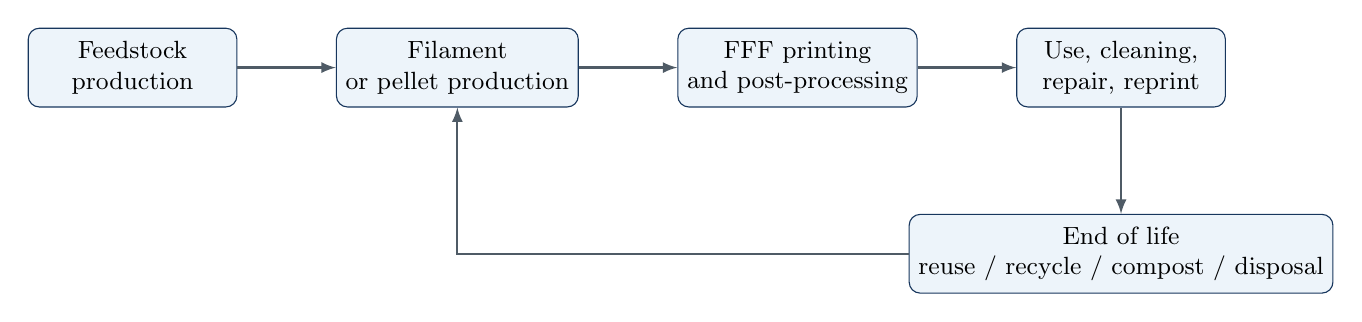
\begin{tikzpicture}[node distance=1.25cm,>=latex,
  box/.style={draw=navy,rounded corners,fill=lightblue,minimum width=2.65cm,minimum height=1.0cm,align=center,font=\small},
  arrow/.style={->,thick,color=slate}]
\node[box] (feed) {Feedstock\\production};
\node[box,right=of feed] (fil) {Filament\\or pellet production};
\node[box,right=of fil] (print) {FFF printing\\and post-processing};
\node[box,right=of print] (use) {Use, cleaning,\\repair, reprint};
\node[box,below=1.35cm of use] (eol) {End of life\\reuse / recycle / compost / disposal};
\draw[arrow] (feed) -- (fil);
\draw[arrow] (fil) -- (print);
\draw[arrow] (print) -- (use);
\draw[arrow] (use) -- (eol);
\draw[arrow] (eol.west) -| (fil.south);
\end{tikzpicture}
\caption{System-level boundary used for sustainability reasoning. The return path represents potential closed-loop material recovery, not an assumption that recycling is always available.}
\label{fig:lifecycle}
\end{figure}

ISO 14040 and ISO 14044 organize LCA around goal and scope definition, inventory, impact assessment, and interpretation \cite{iso14040,iso14044}. For custom assistive devices, the functional unit should ideally represent a delivered function over time, not merely one kilogram of filament or one completed print. This distinction becomes decisive when one material requires frequent replacement or generates a higher failed-print rate.

\subsection{Interpretation rule}

Throughout this report, material recommendations are conditional statements of the form
\begin{equation}
  m^* = \arg\min_{m \in \mathcal{F}} I(m \mid g,p,u,e),
\end{equation}
where $m$ is a candidate material, $\mathcal{F}$ is the set of materials satisfying hard feasibility constraints, $g$ denotes part geometry, $p$ process settings, $u$ the user/service environment, and $e$ the local energy and end-of-life context. The equation is not a complete LCA model; it makes explicit why a universal ranking of PLA, PETG/rPETG, and PHA is generally not defensible.

% ---------------- DESIGN CONTEXT ----------------
\section{Design Context: 3D-Printed Assistive Devices}

Assistive devices create a distinctive material-selection problem. A prototype may be printed in hours, but the user may depend on the final part during cooking, writing, exercise, communication, or daily mobility. The relevant functional unit is therefore not simply ``one printed part.'' A more defensible functional unit is closer to \emph{one successful function delivered over a defined service period}.

\subsection{Key engineering requirements}

For low-cost custom assistive devices, the following requirements should be considered explicitly:

\begin{itemize}
  \item \textbf{Fit and customization}: geometry must reflect the user's body, grip, reach, range of motion, or attachment interface.
  \item \textbf{Mechanical reliability}: the device must withstand expected loads, impacts, and repeated cycles with a suitable safety margin.
  \item \textbf{Comfort}: sharp edges, local pressure concentrations, excessive stiffness, and poor surface finish can reduce usability.
  \item \textbf{Moisture and cleaning}: kitchen tools, exercise aids, and daily-wear devices may be exposed to sweat, water, soaps, or disinfectants.
  \item \textbf{Repair and reprint}: digital files can enable low-cost replacement, but design modularity determines whether the entire device must be reprinted after a local failure.
  \item \textbf{Safe failure}: a material that fails gradually or visibly may be preferable to one that fails abruptly in a load-bearing application.
\end{itemize}

The literature on additively manufactured orthoses, prostheses, and other assistive technologies emphasizes customization and low-volume fabrication while also identifying mechanical integrity, fit, qualification, and clinical validation as persistent challenges \cite{chen2016,tenkate2017,sakib2023,rasmussen2026}. A recent review of user-centered 3D-printed assistive devices further supports integrating user requirements before and during development rather than using usability evaluation only after fabrication \cite{coelho2026}.

\begin{cautionbox}{Important scope boundary}
This report does not certify any filament for clinical, medical, food-contact, or prolonged skin-contact use. Material suitability depends on the exact device, polymer grade, additives, printer hardware, surface finish, cleaning protocol, and applicable regulation. The recommendations here are engineering screening guidance for prototyping and design selection.
\end{cautionbox}

% ---------------- MATERIALS ----------------
\section{Material Families}

\subsection{PLA}

PLA is a bio-based aliphatic polyester commonly produced from fermented carbohydrate feedstocks. Its practical advantages in desktop FFF include low warpage, relatively easy process control, and lower required thermal input than many engineering thermoplastics. These characteristics make PLA particularly attractive for rapid prototyping and geometry iteration.

From a sustainability perspective, PLA's renewable feedstock does not automatically guarantee low total impact. Printing energy, failed builds, transportation, additives, electricity mix, and actual end-of-life handling remain important. Industrial compostability claims also depend on controlled facility conditions and certification; they should not be interpreted as rapid degradation in ordinary soil, home compost, or landfill environments \cite{astmd6400,sola2024}.

\textbf{Assistive-device implication.} PLA is a strong prototyping material for fit checks, handles, jigs, lightweight holders, and non-critical components. Its lower heat resistance and relatively brittle failure behavior can be limiting for hot environments, impact loading, repeated flexure, or parts left in vehicles.

\subsection{PETG and recycled PET-based feedstocks}

PETG is valued in FFF for toughness, layer adhesion, moisture resistance, and functional durability. Recycled PET-based feedstocks can reduce reliance on virgin resin and create a pathway for higher-value reuse of waste plastics. Zander et al. demonstrated the technical feasibility of processing reclaimed PET packaging into FFF feedstock, illustrating the potential of distributed recycling for additive manufacturing \cite{zander2018}.

Circularity is still a systems problem. Material sorting, contamination, moisture control, extrusion consistency, and repeated thermal history can affect print quality and mechanical behavior. Recycled content should therefore be accompanied by traceability and quality control rather than treated as an automatic environmental advantage.

\textbf{Assistive-device implication.} PETG/rPETG is often a stronger candidate than PLA for durable handles, clips, holders, moisture-exposed parts, and devices that receive repeated handling. Its longer service life can compensate for a higher per-print energy requirement if it reduces breakage and replacement frequency.

\subsection{PHA}

PHAs are microbial polyesters produced by a wide range of organisms. They are attractive because they can be bio-based and because many PHA grades can biodegrade under a broader set of conditions than PLA. Current research also investigates production from waste-derived feedstocks, potentially linking biopolymer production to circular-economy strategies \cite{zhou2023,getino2024}.

However, PHA is not one material. Properties vary substantially across grades and copolymer compositions. Cost, brittleness in some grades, processing windows, and supply consistency remain important barriers. Biodegradation rate also depends on polymer chemistry, temperature, moisture, geometry, microbial environment, additives, and crystallinity \cite{zhou2023,dhaini2024,derippe2024,read2024}. Recent marine field studies reinforce that even within the PHA family, degradation kinetics are strongly environment- and formulation-dependent; ``biodegradable should therefore be treated as a testable condition, not an unconditional disposal claim \cite{read2024,derippe2024}.

\textbf{Assistive-device implication.} PHA is most compelling when environmental leakage risk is itself a design driver or when a specific PHA grade offers a useful mechanical/biocompatibility profile. It is not yet the obvious default for general low-cost assistive-device fabrication.

\subsection{Comparative engineering summary}

\begin{table}[htbp]
\centering
\small
\caption{Qualitative comparison for FFF prototyping and low-volume assistive-device fabrication. Rankings synthesize the reviewed literature and engineering requirements; they are not standardized material test results.}
\begin{tabularx}{\textwidth}{@{}lYYY@{}}
\toprule
\textbf{Criterion} & \textbf{PLA} & \textbf{PETG / rPETG} & \textbf{PHA} \\
\midrule
Printability & Very good; forgiving for prototypes & Good; requires more thermal control & Grade-dependent; often narrower window \\
Toughness & Moderate; can be brittle & High relative to PLA & Variable; grade-dependent \\
Moisture resistance & Limited to moderate & Good & Variable \\
Heat tolerance & Limited & Better than PLA in many uses & Grade-dependent \\
Recycled-feedstock pathway & Possible but sorting is limited & Strong potential through PET-derived streams & Emerging; focus is often bio/waste feedstocks \\
Biodegradation potential & Mainly industrial composting for certified grades & Low & Potentially broad, grade/environment dependent \\
Cost / availability & Excellent & Very good & Currently weaker \\
Best portfolio use case & Prototypes, fit checks, light-duty aids & Durable functional aids and repeated handling & Research / leakage-sensitive applications \\
\bottomrule
\end{tabularx}
\end{table}

% ---------------- MANUFACTURING MECHANICS ----------------
\section{Manufacturing--Structure--Property Coupling}

Material selection cannot be separated from process selection because FFF produces a mesostructured, anisotropic component rather than an isotropic bulk-polymer specimen. Inter-bead bonding, void content, raster direction, build orientation, extrusion temperature, layer thickness, infill, and local toolpath geometry change both stiffness and failure behavior \cite{chacon2017,cojocaru2022}. This point is central to assistive devices, where the direction of an applied grip, bending moment, strap load, or impact may be predictable enough to orient the printed structure intentionally.

\subsection{Anisotropy as a design variable}

A useful engineering abstraction is to separate in-plane strength from through-layer strength. If the principal service load is $\mathbf{F}$ and the printed material has orientation-dependent strength $\sigma_u(\theta)$, a first screening requirement is
\begin{equation}
  \sigma_{\mathrm{eq}}(\mathbf{F},g) \leq \frac{\sigma_u(\theta,p,m)}{N_s},
\end{equation}
where $g$ is geometry, $p$ is the process parameter set, $m$ the material, and $N_s$ a safety factor selected for the consequence of failure. This expression is intentionally generic: it highlights that the allowable stress belongs to the \emph{printed process-material system}, not only to the polymer datasheet.

Chac{\'o}n et al. demonstrated strong dependence of PLA mechanical performance on build orientation, layer thickness, and feed rate, and later reviews confirm that raster orientation and build direction are major contributors to FFF anisotropy \cite{chacon2017,cojocaru2022}. For a custom aid, geometry optimization without orientation control can therefore produce a nominally efficient design whose weakest interface lies along the dominant service load.

\subsection{Failure consequence and qualification depth}

Not every assistive device requires the same validation depth. A pencil holder and a weight-training hook may use the same printer and polymer but should not share the same qualification logic. The appropriate test burden increases with load, cyclic exposure, proximity to the body, and consequence of failure.

\begin{table}[htbp]
\centering
\small
\caption{Risk-informed qualification levels for custom FFF assistive devices.}
\begin{tabularx}{\textwidth}{@{}p{0.18\textwidth}p{0.27\textwidth}YY@{}}
\toprule
\textbf{Level} & \textbf{Example} & \textbf{Primary concern} & \textbf{Recommended evidence} \\
\midrule
Low & Pencil/stylus holder, light phone stand & Fit, comfort, dimensional stability & User fit check, visual inspection, simple static proof load if relevant \\
Moderate & Adaptive utensil interface, guitar-pick holder & Repeated handling, moisture, localized stress & Repeated-use testing, cleaning exposure, orientation review, proof loading \\
High & Exercise attachment or load-bearing hook & Sudden failure, fatigue, large force & Standardized material coupons, device-level proof/fatigue tests, documented safety factor, retirement criteria \\
\bottomrule
\end{tabularx}
\end{table}

For research-grade characterization, ASTM D638 tensile testing, ASTM D790 flexural testing, and ASTM D256 impact testing provide standardized baselines for plastic materials \cite{astmd638,astmd790,astmd256}. These coupon tests do not replace device-level validation because local stress concentrations, print orientation, fasteners, straps, and user interaction can dominate actual failure.

\subsection{Moisture, cleaning, and chemical exposure}

Assistive devices used in kitchens, exercise environments, or daily wear may experience water, sweat, detergents, alcohol-based cleaners, oils, or food residues. Chemical exposure can alter mass, dimensions, surface condition, and mechanical properties; ASTM D543 provides a standardized framework for comparative chemical-resistance evaluation \cite{astmd543}. A graduate-level material-selection argument should therefore distinguish bulk mechanical performance from retained performance after realistic conditioning.

% ---------------- LCA ----------------
\section{Life-Cycle Assessment and the Problem with Single-Label Sustainability}

The environmental performance of FFF is highly sensitive to system boundaries. A cradle-to-gate comparison of resin production can produce a different ranking from a cradle-to-grave comparison that includes printing electricity, failed prints, use duration, repair, and disposal. Recent LCA literature on FFF identifies energy consumption and process time as recurring drivers of environmental impact \cite{sola2024}.

\subsection{Functional unit}

A useful functional unit for assistive-device comparison might be:

\begin{equation}
\text{Impact per service} = \frac{I_{\mathrm{feedstock}} + I_{\mathrm{printing}} + I_{\mathrm{post}} + I_{\mathrm{EOL}}}{N_{\mathrm{successful\ uses}}}
\end{equation}

This expression is conceptual rather than a complete LCA model. Its purpose is to emphasize that durability and successful use matter. A slightly higher-impact material can have a lower impact per successful use if it lasts substantially longer or reduces reprints.

A more explicit service-normalized formulation can include yield and replacement frequency:
\begin{equation}
I_{\mathrm{service}} = \frac{I_{\mathrm{mat}}+I_{\mathrm{print}}+I_{\mathrm{post}}+I_{\mathrm{transport}}+I_{\mathrm{EOL}}}{Y_{\mathrm{print}}\,L_{\mathrm{service}}},
\end{equation}
where $Y_{\mathrm{print}}$ is the probability that a print becomes an acceptable device and $L_{\mathrm{service}}$ is a service-life measure such as successful uses, days, or duty cycles. The formulation prevents a material with nominally low cradle-to-gate burden from appearing favorable if it has a high failure rate or short usable life.

\subsection{Uncertainty and sensitivity}

Published FFF LCA results can disagree because functional units, electricity mixes, machine power, support material, infill, part geometry, and allocation methods differ \cite{sola2024}. Therefore, a single point estimate should not be interpreted as a universal ranking. A more defensible analysis treats uncertain parameters as intervals or distributions and asks whether the ranking is stable under plausible scenarios.

For parameter vector $\boldsymbol{\theta}$, define the pairwise impact difference
\begin{equation}
  \Delta I_{ab}(\boldsymbol{\theta})=I_a(\boldsymbol{\theta})-I_b(\boldsymbol{\theta}).
\end{equation}
If $\Delta I_{ab}$ changes sign across credible scenarios, the evidence supports a \emph{conditional tradeoff}, not a categorical statement that material $a$ is more sustainable than material $b$. For this portfolio review, no Monte Carlo LCA was performed; this equation defines the recommended analytical standard for future work.


\subsection{Design parameters as environmental parameters}

Layer height, infill, support strategy, part orientation, and print speed are not only manufacturing variables; they are also environmental variables. The systematic review by Sola et al. highlights print duration, infill, and electricity as important contributors to FFF impact \cite{sola2024}. This creates a direct connection between mechanical design and sustainability:

\begin{itemize}
  \item excessive infill increases both material consumption and print time;
  \item unnecessary support creates waste without adding service value;
  \item very thin layers improve surface finish but can significantly lengthen printing;
  \item poor orientation can increase support volume and reduce strength along critical load paths;
  \item failed prints have nearly zero functional value but retain most of their material and energy burden.
\end{itemize}

\begin{keybox}{Design implication}
For low-volume assistive devices, one of the most effective sustainability strategies may be to reduce unsuccessful iterations: prototype low-cost geometry early, validate fit with the user, then move to the material and print settings appropriate for final service.
\end{keybox}

% ---------------- ENERGY ----------------
\section{Printing Energy and Process Efficiency}

FFF energy demand includes hot-end heating, bed heating, motors, fans, electronics, and any enclosure or filtration system. The environmental importance of electricity depends on print duration and the local electricity mix. Earlier distributed-manufacturing LCA work showed that low-infill PLA printing could be competitive with conventional production under favorable assumptions, while more recent reviews emphasize that results remain highly case-dependent \cite{kreiger2013,sola2024}.

For a practical makerspace or assistive-technology workshop, the following process hierarchy is useful:

\begin{enumerate}
  \item \textbf{Avoid failed prints}: improve bed preparation, filament drying, calibration, and first-layer consistency.
  \item \textbf{Use only the structure required}: tune wall count and infill to load path rather than selecting high infill by habit.
  \item \textbf{Reduce support}: redesign orientation and geometry where possible.
  \item \textbf{Batch efficiently}: where safe and practical, printing multiple small parts in one controlled job can reduce repeated warm-up overhead.
  \item \textbf{Measure rather than assume}: a plug-in watt meter and slicer time estimate can provide a practical project-level energy metric.
\end{enumerate}

A simple experimental measure is

\begin{equation}
E_{\mathrm{part}} = \int_0^{t_{\mathrm{print}}} P(t)\,dt,
\end{equation}

where $P(t)$ is measured printer power. Reporting both $E_{\mathrm{part}}$ and energy per useful mass or per successful service interval allows a more meaningful comparison than using print time alone.

% ---------------- EMISSIONS ----------------
\section{Print-Time Emissions and Safe Operation}

Desktop FFF can emit ultrafine particles and volatile organic compounds. Stephens et al. documented substantial ultrafine-particle emissions from desktop printers, and Azimi et al. later measured both particles and speciated VOCs across multiple printer/filament combinations \cite{stephens2013,azimi2016}. The U.S. EPA and NIOSH similarly describe emissions as an area requiring practical exposure control \cite{epa3dprinting,niosh2023}.

A key point is that ``bio-based'' does not mean ``emission-free.'' Emissions depend on polymer chemistry, additives, colorants, nozzle temperature, and machine configuration. For small workshops and makerspaces, NIOSH recommends applying the hierarchy of controls, including ventilation and engineering controls such as local exhaust and filtration \cite{niosh2023}.

\subsection{Practical controls}

\begin{itemize}
  \item Prefer enclosed printing when compatible with the material and machine.
  \item Use local exhaust or appropriately designed room ventilation where feasible.
  \item Use high-efficiency particle filtration for ultrafine particles and activated-carbon media for relevant gaseous emissions where appropriate.
  \item Avoid unnecessarily high extrusion temperatures.
  \item Keep printers out of densely occupied, poorly ventilated spaces during long print jobs.
  \item Treat unusual odors, smoke, thermal runaway, or degraded filament as process faults rather than normal operating conditions.
\end{itemize}

% ---------------- EOL ----------------
\section{End-of-Life Pathways and Circularity}

\subsection{Composting is an infrastructure claim, not just a material claim}

ASTM D6400 addresses plastics intended to compost under municipal or industrial aerobic composting conditions. A material's ability to meet an industrial compostability specification should not be generalized to home compost, ambient soil, aquatic environments, or landfill \cite{astmd6400}. For PLA, this distinction is especially important: labeling a part ``compostable'' without access to an appropriate facility can misrepresent the realistic disposal pathway.

\subsection{Mechanical recycling}

Mechanical recycling is attractive because it can retain material value, but FFF introduces practical constraints: mixed colors, mixed polymers, adhesives, embedded hardware, contamination, and repeated thermal history. PET-derived feedstocks have demonstrated promise in recycled filament production, but quality control remains central \cite{zander2018}.

\subsection{Design for repair before design for disposal}

For assistive devices, the highest-value circular strategy may often be extension of useful life. This suggests:

\begin{itemize}
  \item replaceable straps and interfaces;
  \item mechanical fasteners instead of permanent adhesive joints where practical;
  \item modular high-wear components;
  \item standardized screw sizes;
  \item retained CAD files for local reprinting;
  \item material labeling on the device or in the digital record.
\end{itemize}

% ---------------- FRAMEWORK ----------------
\section{Application-Based Material Selection Framework}

The matrix below is designed for early-stage engineering screening, especially for custom devices such as utensil holders, writing aids, guitar-pick holders, exercise attachments, and phone or pencil holders. It is intentionally qualitative because commercial filament grades differ and device requirements vary by user.

\begin{table}[htbp]
\centering
\small
\caption{Application-oriented screening framework.}
\begin{tabularx}{\textwidth}{@{}p{0.24\textwidth}YYY@{}}
\toprule
\textbf{Use condition} & \textbf{PLA} & \textbf{PETG/rPETG} & \textbf{PHA} \\
\midrule
Fast fit/geometry prototype & \textbf{Preferred} & Good & Usually unnecessary \\
Repeated daily handling & Conditional & \textbf{Preferred} & Grade-dependent \\
Moisture / sweat exposure & Conditional & \textbf{Preferred} & Grade-dependent \\
Impact / flexural abuse & Often limited & \textbf{Preferred} & Grade-dependent \\
Low-cost classroom outreach & \textbf{Preferred} & Good & Cost-limited \\
High environmental leakage concern & Weak & Weak & \textbf{Potentially preferred} \\
Closed-loop recycled feedstock objective & Moderate & \textbf{Strong potential} & Emerging \\
Lowest process complexity & \textbf{Preferred} & Good & Variable \\
\bottomrule
\end{tabularx}
\end{table}

\subsection{Constraint-based multi-criteria decision model}

A simple weighted score is useful only after unacceptable materials have been removed. A graduate-level decision process therefore separates \textbf{hard feasibility constraints} from \textbf{soft preferences}. Let $x_m$ denote a material/process option. Define the feasible set
\begin{equation}
\mathcal{F}=\left\{x_m:\; g_j(x_m)\leq 0,\;j=1,\ldots,q\right\},
\end{equation}
where $g_j$ may represent minimum proof strength, allowable deflection, dimensional tolerance, cleaning compatibility, maximum print temperature, or cost ceiling. Options that fail a safety or functional requirement do not receive compensating credit for low environmental impact.

For feasible options, a normalized score can be written as
\begin{equation}
S_m = \sum_{i=1}^{n} w_i r_{im}, \qquad w_i\geq0,\qquad \sum_i w_i=1,
\end{equation}
where $r_{im}\in[0,1]$ is the normalized performance of option $m$ on criterion $i$. Candidate criteria include durability, moisture resistance, printability, user comfort, part cost, failed-print rate, embodied impact, printer energy, recycled content, repairability, and realistic local end-of-life access.

\subsection{Sensitivity analysis of decision weights}

Weighted-sum models can hide subjective assumptions. Therefore, the recommended interpretation is not to report a single ``winning'' material, but to test whether the preferred material changes as high-uncertainty weights vary. For example, if $w_{\mathrm{durability}}$ is increased for a load-bearing device, PETG/rPETG may become more favorable; if $w_{\mathrm{leakage}}$ dominates a leakage-prone application, a suitably characterized PHA grade may become more attractive. The engineering conclusion should report the \emph{decision boundary} at which the ranking changes.

A local sensitivity measure can be written as
\begin{equation}
\frac{\partial (S_a-S_b)}{\partial w_i}=r_{ia}-r_{ib}.
\end{equation}
Criteria with large score differences dominate ranking sensitivity and should receive the most careful measurement or stakeholder discussion.

\subsection{Decision ownership in assistive technology}

The weights in a user-centered device should not be assigned by the engineer alone. Some criteria belong to the user (comfort, appearance, cleaning burden, acceptable stiffness), some to engineering safety (strength, fatigue, thermal limit), and some to organizational or environmental priorities (cost, waste, end-of-life). Reviews of assistive-device development emphasize the importance of incorporating user requirements during development rather than only evaluating a finished artifact \cite{coelho2026,rasmussen2026}. The decision model is therefore best used as a shared record of tradeoffs, not as an automated substitute for user involvement.

% ---------------- FOOD WASTE ----------------
\section{Food-Waste-Derived Composite Filament Concept}

The original report introduced \textbf{FOODres.AI}, a conceptual pathway for converting food-waste-derived fillers into printable biopolymer composites. In the original document, several potential benefits were presented as target hypotheses. In this revision, those claims are explicitly separated from demonstrated evidence.

\subsection{Concept architecture}

\begin{figure}[htbp]
\centering
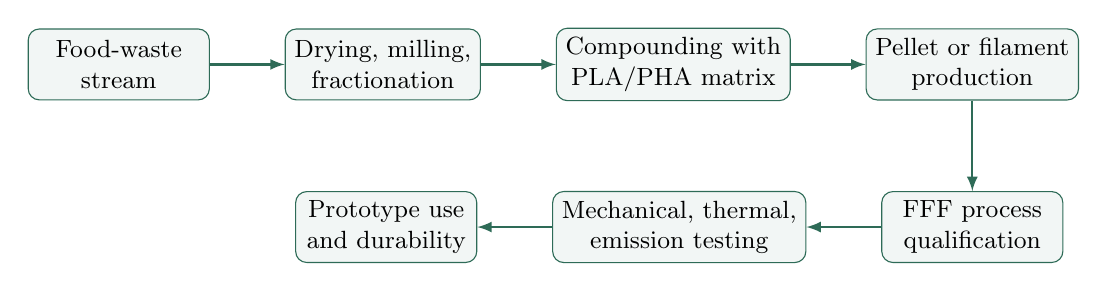
\begin{tikzpicture}[node distance=0.95cm,>=latex,
  box/.style={draw=green,rounded corners,fill=green!6,minimum width=2.3cm,minimum height=0.9cm,align=center,font=\small},
  arrow/.style={->,thick,color=green}]
\node[box] (waste) {Food-waste\\stream};
\node[box,right=of waste] (prep) {Drying, milling,\\fractionation};
\node[box,right=of prep] (comp) {Compounding with\\PLA/PHA matrix};
\node[box,right=of comp] (fil) {Pellet or filament\\production};
\node[box,below=1.15cm of fil] (print) {FFF process\\qualification};
\node[box,left=of print] (test) {Mechanical, thermal,\\emission testing};
\node[box,left=of test] (use) {Prototype use\\and durability};
\draw[arrow] (waste) -- (prep);
\draw[arrow] (prep) -- (comp);
\draw[arrow] (comp) -- (fil);
\draw[arrow] (fil) -- (print);
\draw[arrow] (print) -- (test);
\draw[arrow] (test) -- (use);
\end{tikzpicture}
\caption{Proposed development path for a food-waste-derived composite filament.}
\end{figure}

Waste-derived substrates are already being explored for PHA production and other circular biopolymer routes \cite{zhou2023,getino2024}. However, moving from waste input to reliable FFF feedstock requires control of particle size, moisture, filler-matrix adhesion, viscosity, odor, thermal stability, and diameter consistency.

\subsection{Hypotheses to test, not claims to assume}

A professional development program should treat the following as hypotheses:

\begin{itemize}
  \item adding a waste-derived filler can reduce virgin polymer demand without unacceptable strength loss;
  \item optimized filler content can maintain stable extrusion and interlayer adhesion;
  \item lower processing temperatures may be possible for some formulations, but energy savings must be measured rather than inferred;
  \item waste diversion credits may improve LCA results, but allocation assumptions must be stated explicitly;
  \item odor and emission profiles may change with filler chemistry and require separate measurement.
\end{itemize}

\subsection{Minimum validation program}

\begin{table}[htbp]
\centering
\small
\caption{Proposed validation plan for a food-waste-derived FFF composite.}
\begin{tabularx}{\textwidth}{@{}p{0.23\textwidth}p{0.30\textwidth}Y@{}}
\toprule
\textbf{Question} & \textbf{Measurement} & \textbf{Decision criterion} \\
\midrule
Can it print consistently? & Diameter variation, extrusion stability, failed-print rate, visible defects & Stable feed and repeatable part quality across multiple builds \\
Does it retain function? & Tensile/flexural coupons, interlayer failure, impact screening & Meets device-specific load and safety margin \\
Is it dimensionally stable? & Shrinkage, warpage, dimensional error & Within tolerance required by user fit and attachment geometry \\
Does it save energy? & Watt-meter trace using identical geometry/G-code where possible & Lower measured energy per acceptable part, not just lower nozzle setpoint \\
Are emissions acceptable? & Particle/VOC screening under controlled settings & No unacceptable increase relative to reference material; controls defined \\
Is the sustainability claim real? & Cradle-to-grave LCA sensitivity study & Benefit remains under reasonable allocation, electricity, and EOL scenarios \\
\bottomrule
\end{tabularx}
\end{table}

% ---------------- QUALIFICATION ----------------
\section{Research-Grade Validation Plan}

The original review was literature-based; it did not experimentally rank PLA, rPETG, PHA, or food-waste composites. A graduate-level extension should convert the review into a testable research program with controlled factors, replicates, and predefined decision metrics.

\subsection{Phase I: process window and printability}

A screening design of experiments should first identify a stable processing window for each material. Candidate factors include nozzle temperature, bed temperature, layer height, print speed, raster orientation, and material conditioning. Responses should include extrusion stability, dimensional error, warpage, surface defects, print time, part mass, and failed-print rate. Material comparisons should use equivalent geometries and clearly state whether process parameters are held constant or optimized separately for each material.

\subsection{Phase II: mechanical characterization}

At minimum, tensile and flexural characterization should follow recognized plastic-test frameworks such as ASTM D638 and D790, with impact testing considered for applications where sudden loading is relevant \cite{astmd638,astmd790,astmd256}. Because FFF is anisotropic, specimens should be printed in at least two strategically selected orientations rather than treating one orientation as representative of the process \cite{chacon2017,cojocaru2022}.

For each response $y$, report sample size, mean, standard deviation, confidence interval, and effect size where appropriate. A one-way or factorial ANOVA may be used when assumptions are satisfied; otherwise, robust or nonparametric alternatives should be considered. Statistical significance should not replace engineering significance: a small increase in tensile strength may be irrelevant if the device-level safety factor is already large, whereas a modest improvement in interlayer toughness can be important in a geometry dominated by peel or bending.

\subsection{Phase III: environmental conditioning and device-level testing}

Material coupons should be complemented by the actual assistive-device geometry. Conditioning can include water, sweat surrogate, cleaning agents, thermal cycling, or UV exposure depending on use. ASTM D543 provides a useful framework for comparative chemical exposure \cite{astmd543}. Device-level testing should include the dominant expected load, repeated-use cycles, fastener/strap interfaces, and a documented failure or retirement criterion.

\subsection{Phase IV: energy, emissions, and LCA}

Printer power should be recorded at sufficient temporal resolution to compute
\begin{equation}
E_{\mathrm{part}}=\int_0^{t_f}P(t)\,dt,
\end{equation}
with failed builds included in the yield-adjusted inventory. Emission testing, if available, should be performed under controlled enclosure and ventilation conditions because polymer, additives, temperature, and printer configuration affect ultrafine-particle and VOC emissions \cite{stephens2013,azimi2016,niosh2023}. The LCA should then use the experimentally observed material mass, print yield, energy, and service-life data rather than generic slicer estimates whenever possible.

\subsection{Phase V: user-centered validation}

Engineering qualification should be paired with structured user feedback on task completion, comfort, donning/doffing, cleaning, perceived security, and willingness to use the device. The need for stronger patient-centered outcome evidence in 3D-printed assistive technology is explicit in recent systematic-review literature \cite{rasmussen2026}. For a research study, the protocol should distinguish engineering usability testing from clinical research and obtain appropriate ethics review when human-subjects research criteria are met.

\begin{keybox}{Minimum evidence needed before a sustainability claim}
A material should not be described as the ``more sustainable'' assistive-device option merely because it is recycled, bio-based, or biodegradable. The claim should be supported by: (1) equivalent functional performance, (2) measured or defensible service life, (3) print yield, (4) actual energy/material inventory, (5) realistic local end-of-life assumptions, and (6) sensitivity analysis showing whether the conclusion survives plausible uncertainty.
\end{keybox}

% ---------------- PRACTICAL RECS ----------------
\section{Practical Recommendations for a Small Assistive-Technology Workshop}

The following recommendations translate the literature into an operational workflow appropriate for low-volume, user-centered fabrication.

\subsection{Prototype-to-final workflow}

\begin{enumerate}
  \item \textbf{Define the user's functional need} and likely load/environment before selecting a polymer.
  \item \textbf{Prototype geometry quickly} in an easy-to-print material, often PLA.
  \item \textbf{Validate fit and usability} with the user before increasing infill or moving to a more durable material.
  \item \textbf{Select the final material} based on actual service conditions rather than sustainability labels alone.
  \item \textbf{Orient for strength} along the expected load path and reduce unnecessary supports.
  \item \textbf{Record print settings and material lot} for reproducibility.
  \item \textbf{Inspect before use} and define visible retirement criteria for high-load devices.
  \item \textbf{Design replacement modules} so wear does not require full-device disposal.
\end{enumerate}

\subsection{Material choice by example}

\begin{itemize}
  \item \textbf{Adaptive kitchen utensil holder}: prioritize cleanability, moisture resistance, grip interface, and safe load transfer; PETG/rPETG may be preferable to PLA for repeated wet handling, subject to device-specific validation.
  \item \textbf{Pencil or stylus holder}: low load and high customization make PLA a practical default for geometry iteration and final use if heat exposure is limited.
  \item \textbf{Weight-training hook}: load magnitude and failure consequence dominate sustainability claims; prototype materials should not be treated as validated final-load materials without mechanical testing.
  \item \textbf{Guitar-pick holder}: comfort, fit, low mass, and fatigue around thin features may matter more than bulk tensile strength.
\end{itemize}

% ---------------- DISCUSSION ----------------
\section{Discussion}

The literature points to a recurring methodological problem: material sustainability, manufacturability, and user function are often evaluated in separate studies even though a real assistive device couples all three. FFF makes that coupling unusually strong. A lower-temperature material may reduce printer energy but may require more frequent replacement. A tougher material may have a larger cradle-to-gate burden but lower service-normalized impact. A biodegradable material may reduce persistence if leaked to a suitable environment, but may offer no practical advantage if the actual product enters municipal landfill. Likewise, a recycled feedstock can improve circularity while increasing variability, moisture sensitivity, or failed-print frequency if quality control is insufficient \cite{sola2024,zander2018}.

The strongest conclusion of this review is therefore not a polymer ranking. It is a \textbf{decision architecture}. First, define the user function and failure consequence. Second, eliminate materials and print configurations that do not satisfy mechanical, environmental-exposure, or usability constraints. Third, compare the remaining options using service-normalized environmental metrics. Fourth, test the decision against uncertainty in service life, print yield, electricity mix, and end-of-life access. Finally, document which assumptions came from standards, experiments, literature synthesis, and stakeholder preferences.

This architecture also clarifies the role of ``sustainable design'' in custom assistive technology. Sustainability is not separable from user-centered design because an unused, uncomfortable, unreliable, or difficult-to-clean device has low functional value regardless of its feedstock label. Recent systematic review evidence on 3D-printed assistive technology highlights promising outcomes but also the need for higher-quality patient-centered evidence \cite{rasmussen2026}. User-centered development literature similarly argues for earlier integration of user requirements \cite{coelho2026}. In this sense, durability, acceptance, repairability, and successful task performance are not merely human-factors additions to environmental analysis; they are part of the denominator of meaningful environmental performance.

\subsection{Implications for Humanos 3D-style workflows}

For a small assistive-technology organization, the practical value of this framework is its ability to scale evidence requirements to risk. Low-load geometry prototypes can prioritize speed and fit. Repeated-use functional devices should add conditioning and cyclic tests. High-consequence load-bearing components require much stronger mechanical qualification and should not rely on desktop-FFF material reputation alone. This tiered approach preserves the accessibility and iteration speed that make FFF attractive while reducing the risk of overclaiming safety or sustainability.

% ---------------- GAPS ----------------
\section{Research Gaps and Future Work}

Several gaps remain before sustainability claims for FFF materials in custom assistive technology can be made with high confidence. These gaps are both physical (missing measurements) and methodological (inconsistent functional units, limited user-centered evidence, and weak linkage between mechanical durability and LCA).

\begin{enumerate}
  \item \textbf{Real-world LCA data for small assistive devices.} Published FFF LCAs often use generic coupons or industrial comparisons rather than user-specific devices and reprint/repair cycles.
  \item \textbf{Durability-adjusted environmental metrics.} Material comparisons should account for service life and failure frequency, not only impact per kilogram.
  \item \textbf{Recycled filament quality control.} More data are needed on how repeated processing, moisture, additives, and source variability affect functional performance.
  \item \textbf{Emission profiles across colorants and additives.} NIOSH and EPA guidance show that printer/filament combinations can differ meaningfully, making broad material labels insufficient \cite{niosh2023,epa3dprinting}.
  \item \textbf{PHA grade-specific printing data.} The PHA family is diverse, so biodegradation and mechanical claims require grade-specific evidence \cite{zhou2023,getino2024}.
  \item \textbf{Food-waste composites.} Rheology, odor, filler consistency, mechanical anisotropy, emissions, and end-of-life behavior should be measured under repeatable protocols.
\end{enumerate}

% ---------------- LIMITATIONS ----------------
\section{Limitations}

This review synthesizes heterogeneous evidence rather than conducting a registered systematic review or meta-analysis. The literature search was structured but not exhaustive, so publication-selection bias is possible. In addition, recent 2026 publications were included in this portfolio revision and were not available when the original 2025 internship report was written. The revision should therefore be understood as an updated technical synthesis, not as a time-frozen reproduction of the original document.

 Material properties vary by commercial formulation, additive package, color, moisture history, print orientation, raster pattern, infill, and machine configuration. Therefore, rankings in this document should be understood as screening guidance, not universal material constants.

The report also intentionally avoids converting unvalidated concepts into performance claims. In particular, the FOODres.AI section is a proposal for a research pathway. Any claims regarding tensile strength, energy savings, carbon reduction, biodegradation, or consumer viability would require direct experimental and life-cycle evidence.

Finally, sustainability depends on location. A recycled or compostable pathway only creates real benefit when appropriate collection, processing, and end-of-life infrastructure actually exist.

% ---------------- CONCLUSION ----------------
\section{Conclusion}

Sustainable material selection for FFF is a multi-objective engineering decision. PLA, PETG/rPETG, and PHA each offer different strengths, but no polymer is environmentally preferable under all conditions. A defensible choice must consider feedstock, printing energy, emissions, mechanical performance, expected service life, repairability, user context, and realistic end-of-life infrastructure.

For assistive-device prototyping, PLA remains an efficient starting point because it is accessible and easy to print. For longer-lived functional devices exposed to moisture, impact, or repeated handling, PETG or recycled PET-derived feedstocks can be attractive when quality and recycling pathways are controlled. PHA offers distinctive biodegradation potential but currently requires more careful grade selection and economic justification.

The most important design lesson is broader than any one filament: \textbf{sustainability is a property of a functioning product system, not a material label.} A lower-impact assistive device must work reliably, survive an appropriate service life, be accepted and usable by the person it is designed for, avoid unnecessary print failures, be repairable when practical, and enter an end-of-life pathway that actually exists. The engineering standard should therefore shift from asking ``Which filament is greenest? to asking ``Which feasible material--process--design combination delivers the required human function with the lowest robust service-normalized burden under realistic uncertainty?

\newpage
\printbibliography[title={References}]

\end{document}
